% !TEX TS-program = lualatex
% !TEX encoding = UTF-8 Unicode		

\documentclass[12pt, letterpaper]{article}

%%BIBLIOGRAPHY- This uses biber/biblatex to generate bibliographies according to the 
%%Unified Style Sheet for Linguistics
\usepackage[main=american, german]{babel}% Recommended
\usepackage{csquotes}% Recommended
\usepackage[backend=biber,
		style=unified,
		maxcitenames=3,
		maxbibnames=99,
		natbib,
		url=false]{biblatex}
\addbibresource{../Library.bib}
\setcounter{biburlnumpenalty}{100}  % allow URL breaks at numbers
%\setcounter{biburlucpenalty}{100}   % allow URL breaks at uppercase letters
%\setcounter{biburllcpenalty}{100}   % allow URL breaks at lowercase letters

%%TYPOLOGY
\usepackage[svgnames]{xcolor} % Specify colors by their 'svgnames', for a full list of all colors available see here: http://www.latextemplates.com/svgnames-colors
%\usepackage[compact]{titlesec}
%\titleformat{\section}[runin]{\normalfont\bfseries}{\thesection.}{.5em}{}[.]
%\titleformat{\subsection}[runin]{\normalfont\scshape}{\thesubsection}{.5em}{}[.]
\usepackage[hmargin=1in,vmargin=1in]{geometry}  %Margins          
\usepackage{graphicx}	%Inserting graphics, pictures, images 		
\usepackage{stackengine} %Package to allow text above or below other text, Also helpful for HG weights 
\usepackage{fontspec} %Selection of fonts must be ran in XeLaTeX or LuaLaTeX
\usepackage{amssymb} %Math symbols
\usepackage{amsmath} % Mathematical enhancements for LaTeX
\usepackage{setspace} %Linespacing
\usepackage{multicol} %Multicolumn text
\usepackage{enumitem} %Allows for continuous numbering of lists over examples, etc.
\usepackage{multirow} %Useful for combining cells in tablesbrew 
\usepackage{booktabs}
\usepackage{hanging}
\usepackage{fancyhdr} %Allows for the 
\pagestyle{fancy}
\fancyhead[L]{\textit{QP Handout}} 
\fancyhead[R]{\textit{\today}} 
\fancyfoot[L,R]{} 
\fancyfoot[C]{\thepage} 
\renewcommand{\headrulewidth}{0.4pt}
\setlength{\headheight}{14.5pt} % ...at least 14.49998pt
% \usepackage{fourier} % This allows for the use of certain wingdings like bombs, frowns, etc.
% \usepackage{fourier-orns} %More useful symbols like bombs and jolly-roger, mostly for OT
\usepackage[colorlinks,allcolors={black},urlcolor={blue}]{hyperref} %allows for hyperlinks and pdf bookmarks
% \usepackage{url} %allows for urls
% \def\UrlBreaks{\do\/\do-} %allows for urls to be broken up
\usepackage[normalem]{ulem} %strike out text. Handy for syntax
\usepackage{tcolorbox}
\usepackage{datetime2}

%%FONTS
\setmainfont{Libertinus Serif}
\setsansfont{Libertinus Sans}
\setmonofont[Scale=MatchLowercase]{Libertinus Mono}

%%PACKAGES FOR LINGUISTICS
%\usepackage{OTtablx} %Generating tableaux with using TIPA
\usepackage[noipa]{OTtablx} % Use this one generating tableaux without using TIPA
%\usepackage[notipa]{ot-tableau} % Another tableau drawing packing use for posters.
% \usepackage{linguex} % Linguistic examples
% \usepackage{langsci-linguex} % Linguistic examples
\usepackage{langsci-gb4e} % Language Science Press' modification of gb4e
% \usepackage{langsci-avm} % Language Science Press' AVM package
\usepackage{tikz} % Drawing Hasse diagrams
% \usepackage{pst-asr} % Drawing autosegmental features
\usepackage{pstricks} % required for pst-asr, OTtablx, pst-jtree.
% \usepackage{pst-jtree} 	% Syntax tree draawing software
% \usepackage{tikz-qtree}	% Another syntax tree drawing software. Uses bracket notation.
\usepackage[linguistics]{forest}	% Another syntax tree drawing software. Uses bracket notation.
% \usepackage{ling-macros} % Various linguistic macros. Does not work with linguex.
% \usepackage{covington} % Another linguistic examples package.
\usepackage{leipzig} %	Offers support for Leipzig Glossing Rules

%%LEIPZIG GLOSSING FOR ZAPOTEC
\newleipzig{el}{el}{elder}	% Elder pronouns
\newleipzig{hu}{hu}{human}	% Human pronouns
\newleipzig{an}{an}{animate}	% Animate pronouns
\newleipzig{in}{in}{inanimate}	% Inanimate pronouns
\newleipzig{pot}{pot}{potential}	% Potential Aspect
\newleipzig{cont}{cont}{continuative}	% Continuative Aspect
% \newleipzig{pot}{pot}{potential}	% Potential Aspect
\newleipzig{stat}{stat}{stative}	% Potential Aspect
\newleipzig{and}{and}{andative}	% Andative Aspect
\newleipzig{ven}{ven}{venative}	% Venative Aspect
% \newleipzig{res}{res}{restitutive}	% Restitutive Aspect
\newleipzig{rep}{rep}{repetitive}	% Repetitive Aspect

%%TITLE INFORMATION
\title{TITLE}
\author{Mykel Loren Brinkerhoff}
\date{\today}

%%MACROS
\newcommand{\sub}[1]{\textsubscript{#1}}
\newcommand{\supr}[1]{\textsuperscript{#1}}
\providecommand{\lsptoprule}{\midrule\toprule}
\providecommand{\lspbottomrule}{\bottomrule\midrule}
\newcommand{\fittable}[1]{\resizebox{\textwidth}{!}{#1}}

\makeatletter
\renewcommand{\paragraph}{%
  \@startsection{paragraph}{4}%
  {\z@}{0ex \@plus 1ex \@minus .2ex}{-1em}%
  {\normalfont\normalsize\bfseries}%
}
\makeatother
\parindent=10pt


\begin{document}
	
%%If using linguex, need the following commands to get correct LSA style spacing
%% these have to be after  \begin{document}
	% \setlength{\Extopsep}{6pt}
	% \setlength{\Exlabelsep}{9pt}		%effect of 0.4in indent from left text edge
%%
	
%% Line spacing setting. Comment out the line spacing you do not need. Comment out all if you want single spacing.
%	\doublespacing
%	\onehalfspacing
	
\begin{center}
	{\Large \textbf{Investigating the timing of tone and phonation in Santiago Laxopa Zapotec}}\footnote{I am grateful to Fe Silva-Robles and  Raúl Díaz Robles for sharing their time and language expertise. I am also grateful to Grant McGuire,  Jaye Padgett, Rachel Walker, Maziar Toosarvandani, Ben Eischens, Kim Tan, and Zach Horton for their help and discussions during all stages of this project. This project branched off from a collaboration with  Jack Duff and Maya Wax Cavallaro. Various parts of this project were previously shared in joint presentations with Jack Duff and Maya Wax Cavallaro.
	
	This work was supported in part the National Science Foundation under Grant No. 2019804, the Humanities Institute at UC Santa Cruz, and the Jacobs Research Funds.}
	\vspace{6pt}

	Mykel Loren Brinkerhoff
\end{center}
%\maketitle
%\maketitleinst
\thispagestyle{fancy}

% \tableofcontents


%------------------------------------
\section{Introduction} \label{sec:Introduction}
%------------------------------------


Most work on the interaction of tone and phonation has been based on descriptions of southeast and far east Asian languages.
This lead to strong claims on the interaction between tone and phonation \citep{masicaDefiningLinguisticArea1976,thurgoodVietnameseTonogenesisRevising2002,yipTone2002,enfieldArealLinguisticsMainland2005,michaudComplexTonesEast2012,brunelleTonePhonationSoutheast2016}.
Main claim from these authors is that tone and phonation are codependent. This is often referred to as a register system.  
Meaning that we only observe certain tones with certain phonations. 
Mandarin Tone 3 is always associated with creaky voice \citep{duanmuPhonologyStandardChinese2007}.
This claim has also been made in the reverse that certain phonation types are associated with specific tonal patterns. 
Breathy voice stereotypically appears with high pitch and creaky voice stereotypically appears with low pitch \citep{eslingVoiceQualityLaryngeal2019}.
This is often born out with research into register systems. 
Also found in pathological voice quality \citep{klattAnalysisSynthesisPerception1990,titzePrinciplesVoiceProduction2000,eslingVoiceQualityLaryngeal2019}.

Research into Mesoamerican languages, however, shows that these claims are too strong or exaggerated \citep{suarezMesoamericanIndianLanguages1983,campbellMesoAmericaLinguisticArea1986,silvermanLaryngealComplexityOtomanguean1997,dicanioPhoneticsPhonologySan2008,espositoVariationContrastivePhonation2010, campbellOtomangueanHistoricalLinguistics2017a,campbellOtomangueanHistoricalLinguistics2017}. 
Most languages of the Oto-Manguean language family exhibits independent tone and phonation.
Tone and phonation freely co-occur or exhibit a much freer distribution than what is found in register languages. San Lucas Quiaviní Zapotec is one such example.


\begin{itemize}
	\item This paper adds to this debate by:
	\begin{itemize}
		\item Providing another description of a language that uses tone and phonation
		\item Evaluates the claims of \citet{silvermanLaryngealComplexityOtomanguean1997}
	\end{itemize}
\end{itemize}

%------------------------------------
\section{The Laryngeal Complexity Hypothesis} \label{sec:Silverman}
%------------------------------------

The \textsc{Laryngeal Complexity Hypothesis} (LCH) has it origins in the work from \citet{silvermanLaryngealComplexityOtomanguean1997,blankenshipTimeCourseBreathiness1997,blankenshipTimingNonmodalPhonation2002}. The basic premise of the LCH is that in languages that have both tone and phonation there needs to be a strict ordering between the laryngeal gestures for tone and phonation. This premise comes from the understanding that the same mechanism that is responsible for tone is also responsible for the production of phonation. The mechanism that is assumed to be responsible is the vocal folds and glottis. The rate that vocal folds vibrate is responsible for changing the frequency that the sound is produced at. This is often perceived as pitch and when pitch is lexicalized it becomes tone. The faster the vocal folds vibrate the higher the pitch and the slower the vocal folds vibrate the lower the pitch. 

The notion that the vocal folds and glottis are responsible for phonation comes from work by \citet{ladefogedPreliminariesLinguisticPhonetics1971,gordonPhonationTypesCrosslinguistic2001} which treated phonation as a by-product of how open or closed the glottis is during vocal fold vibration. This is schematized by Figure~\ref{fig:Phonation}. The more open the glottis is the breathier the sound to the point where the sound becomes the sound [h]. The more closed the glottis is the creakier the sound is to the point where the sound becomes [ʔ]. 
\begin{figure}[!ht]
	\centering
	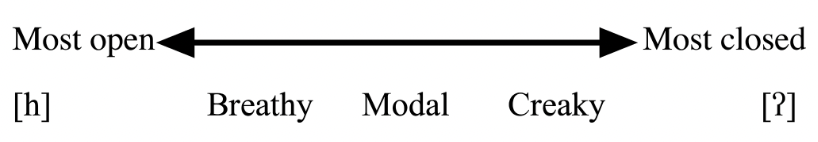
\includegraphics[width=.6\textwidth]{../Phonation.png}
	\caption{Simplified one-deminsional model for phonation. Based on \citet{ladefogedPreliminariesLinguisticPhonetics1971,gordonPhonationTypesCrosslinguistic2001}}.
	\label{fig:Phonation}
\end{figure}
\vspace{-2ex}

The LCH assumes that phonation and tone are both produced at the vocal folds anf glottis. Because these same organs are responsible for these two different phenomena there is a mismatch in trying to produce both at the same time. It is assumed by the LCH that because of this issue there needs to be a strict ordering in the glottal gestures. This means that the tonal gesture needs to be produced either before or after the phonation gesture. The reason for this is that if the gestures were overlapped there will be a perturbation of the tone and the listeners will not be able to reliably differentiate what the tone is. The LCH does assume that there is a close link between production and perception. Primarily, this means that it is burden of the speaker to produce both the tone and phonation gestures in a way that is the most perceptually salient. The assumptions of the LCH is schematized in Figure~\ref{fig:GlottalGestures}.

\begin{figure}[!ht]
	\centering
	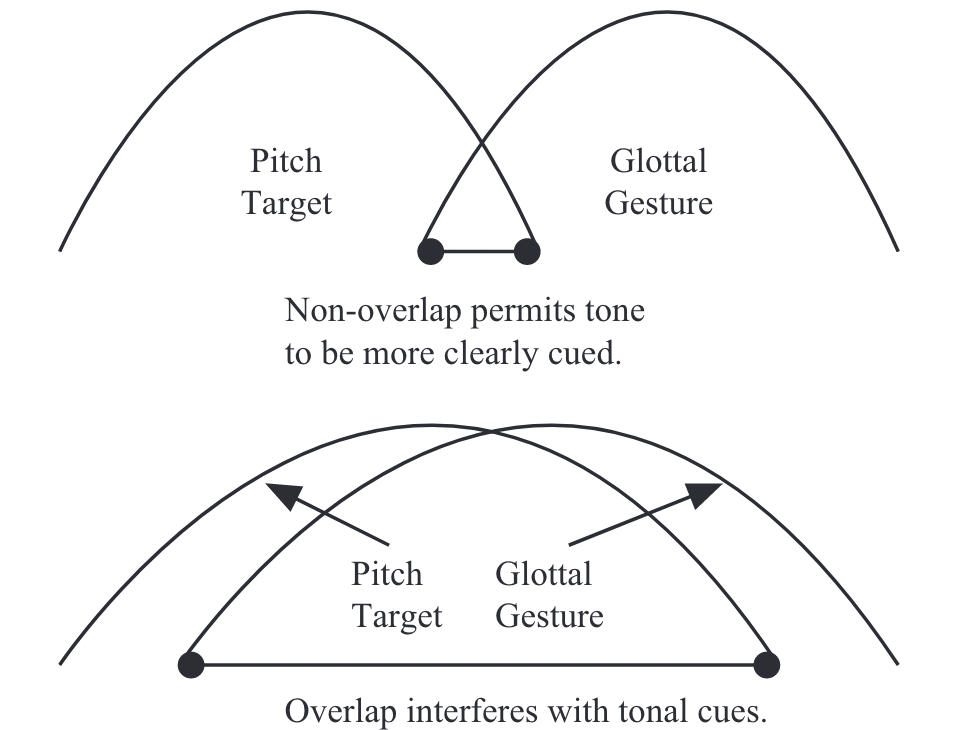
\includegraphics[width=.5\textwidth]{../Gestures.png}
	\label{fig:GlottalGestures}
	\caption{Representation taken from \citet{dicanioCoarticulationToneGlottal2012}.}
\end{figure}

Some work has been done into investigating this in other languages, most notably \posscitet{dicanioCoarticulationToneGlottal2012} investigation into glottals in Itunyoso Trique. \citeauthor{dicanioCoarticulationToneGlottal2012} found that when there is a large degree of overlap in the signal then the acoustic signal for F0 had perturbation. If, however, the degree of overlap was minor then the acoustic signal had no perturbation. In Itunyoso Trique, \citeauthor{dicanioCoarticulationToneGlottal2012} found that there was a statistically significant amount of perturbation throughout the vowel. Another study on Jalapa Mazatec \citep{garellekAcousticConsequencesPhonation2011} also investigated the interaction of tone and phonation. Jalapa Mazatec is a language with both contrastive tone and phonation and \citet{garellekAcousticConsequencesPhonation2011} validated the claims made by the LCH, in that tone and phonation seemed to be ordered with each other when it comes to at least one of the phonation types.

In testing the claims made by the LCH, this paper investigates the interaction of tone and phonation in the Northern Zapotec language of Santiago Laxopa Zapotec. This language is ideal for testing the viability of the LCH because of its use of both contrastive tone and phonation. The rest of the paper will provide a description of the language in Section~\ref{sec:SLZ} with special emphasis on the tone and phonation systems. Following this discussion on Santiago Laxopa Zapotec, this paper discusses an acoustic analysis of phonation modelled on \citet{espositoVariationContrastivePhonation2010,garellekAcousticConsequencesPhonation2011,dicanioCoarticulationToneGlottal2012} in Section~\ref{sec:Acoustics}.

%------------------------------------
\section{Santiago Laxopa Zapotec} \label{sec:SLZ}
%------------------------------------

Santiago Laxopa Zapotec (SLZ; Dilla'xhonh Laxup) is a Northern Zapotec language spoken by approximately 1000 people in the municipality of Santiago Laxopa, Ixtlán District in the Sierra Norte of Oaxaca, Mexico \citep{adlerAcousticsPhonationTypes2016,adlerDerivationVerbInitiality2018,foleyForbiddenCliticClusters2018,foleyExtendingPersonCaseConstraint2020}. It is closely related to San Bartolomé Zoogocho Zapotec \citep{longDiccionarioZapotecoSan2005,sonnenscheinDescriptiveGrammarSan2005} and is mutually intelligible with this variety according to native speakers.  As is common among Zapotecan languages, SLZ distinguishes between lenis and fortis consonants \citep[e.g.,][]{nellisFortisLenisCajonos1980,jaegerFortisLenisQuestion1983,uchiharaFortisLenisGlides2016} and has a fairly standard five-vowel inventory. These contrasts and inventories can be seen in Table~\ref{tab:SLZcons} and Table~\ref{tab:SLZvowels}.


\begin{table}[!h]
	\centering
	\caption{Consonant inventory for Santiago Laxopa Zapotec}
	\label{tab:SLZcons}
	\fittable{
	 \begin{tabular}{llcccccccc}
	  \lsptoprule
		  &  & bilabial & alveolar  & retroflex & alveo- & palatal &velar &labio-  &  uvular \\
		 &&&&& palatal &&&velar& \\
	  \midrule
		nasal    	& lenis   &	   & n  & & & & & & \\
					& fortis  &	mː & nː & & & & & & \\
		stop 		& lenis   & b  & d  & & & & g & gʷ & \\
					   & fortis  & p  & t  & & & & k & kʷ & \\
		fricative   & lenis   &    & z  & ʐ\textasciitilde ɽ & ʒ & ç & &  & ʁ\textasciitilde χ \\
					   & fortis  &    & s  & ʂ & ʃ & & & & \\
		  affricate 	& lenis   &    & d͡z & & & & & & \\
					  & fortis  &    & t͡s & & t͡ʃ & & & & \\
		lateral  	& lenis   &    & l\textasciitilde ɾ & & & & & & \\
					& fortis  &    & lː & & & & & & \\
		trill		& 		  &    & r & & &  & &  & \\ 			
		approximate & 		  &    & & & & j & & w & \\ 
	  \lspbottomrule
	 \end{tabular}
	 }
	\end{table}

	\begin{table}[!h]
		\centering
		\caption{Vowels inventory in Santiago Laxopa Zapotec.}
		\label{tab:SLZvowels}
		 \begin{tabular}{lccc}
		  \lsptoprule
					&  front& central  & back \\
		  \midrule
			high   	&  i  &     &   u \\
			mid    	&  e  &   	& 	o \\
			low   	&     &  a 	&	  \\
		  \lspbottomrule
		 \end{tabular}
		\end{table}
		
In addition to the contrasts in both consonants and vowels, SLZ additionally has a phonation and tonal contrast. I will first talk about the phonation contrasts in Section~\ref{sec:Phonation} followed by the tonal contrasts in Section~\ref{sec:Tone}.

%------------------------------------
\subsection{Phonation in SLZ} \label{sec:Phonation}
%------------------------------------

Among Zapotecan languages it is quite common for languages to make use of contrastive phonation \citep[e.g.,][]{avelinobecerraTopicsYalalagZapotec2004,longDiccionarioZapotecoSan2005,avelinoAcousticElectroglottographicAnalyses2010,lopeznicolasEstudiosFonologiaGramatica2016,chavez-peonInteractionMetricalStructure2010}. 
SLZ, in addition to the five vowel qualities, has four contrastive phonation types which are: modal, breathy, checked, and laryngealized. These contrasts are exemplified in the minimal quadruple in (\ref{ex:YA}). 

\ea \label{ex:YA} Four-way minimal phonation contrast
	\ea \textit{ya} [ja\supr{L}]	`bell'
	\ex \textit{yah}  [ja̤\supr{L}] `metal/rifle'
	\ex \textit{ya'}  [jaˀ\supr{L}]  `pound'
	\ex \textit{ya'a}  [jaˀa\supr{L}]  `market'
	\z 
\z 

Breathy phonation on vowels is characterized by a raspy quality throughout the whole vowel or a portion toward the end of the vowel, see Figure~\ref{fig:BreathyVowel}. 

\begin{figure}[!h]
	\centering
	% [INSERT YAH SPECTROGRAM AND WAVEFORM]
	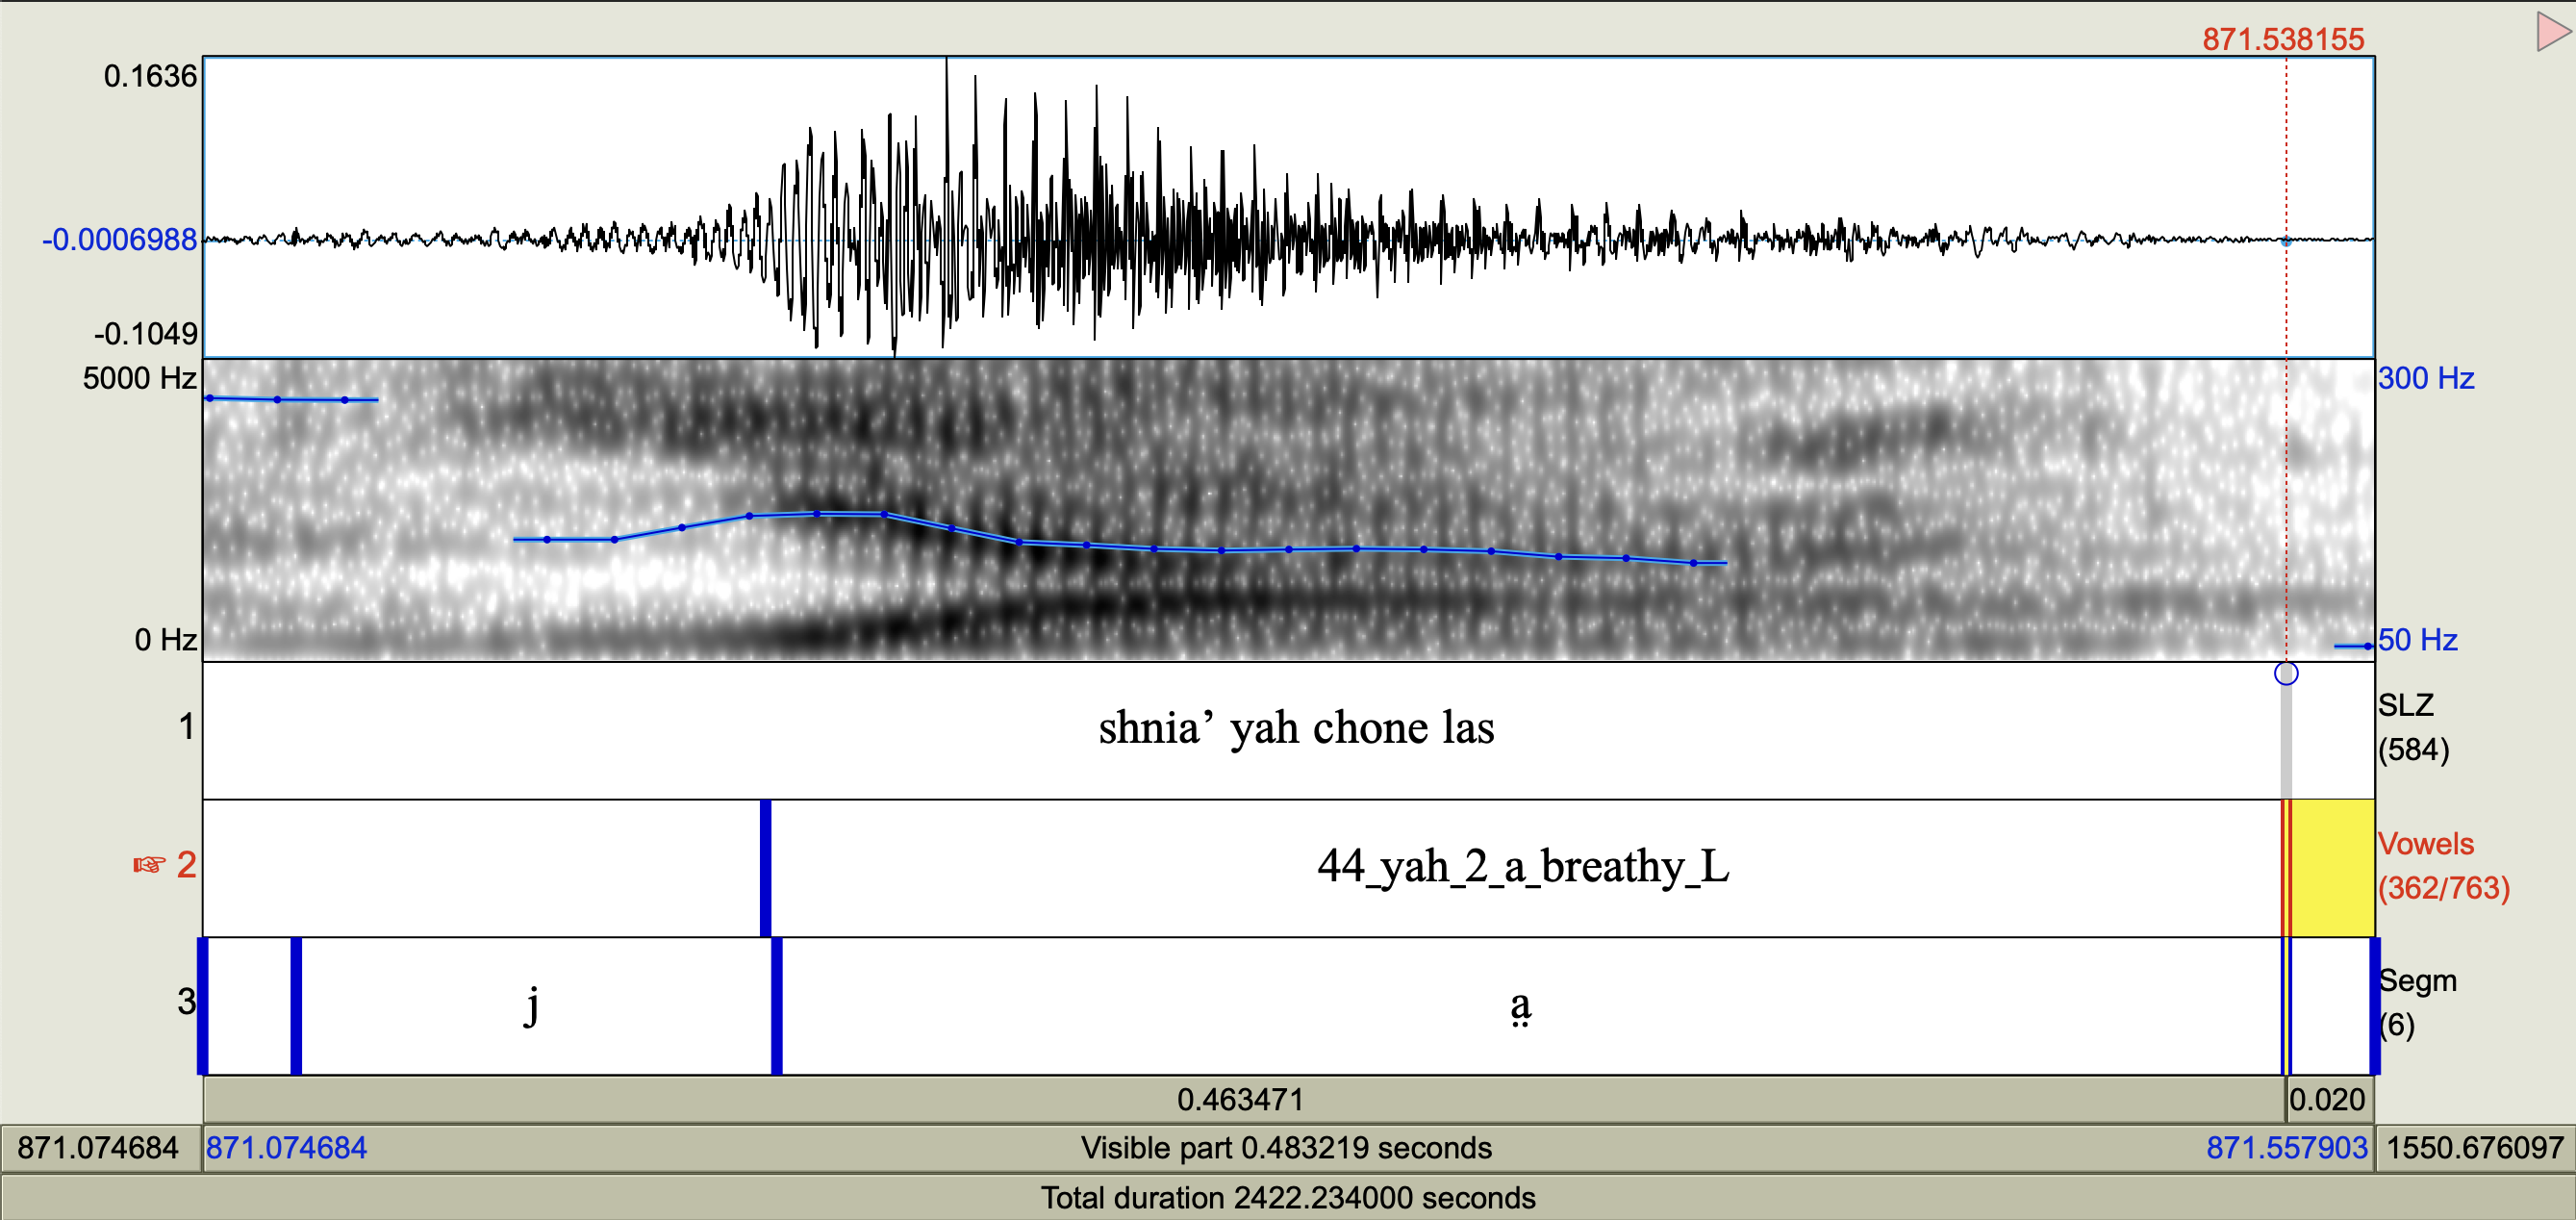
\includegraphics[width=0.9\textwidth]{../yah.png}
	\caption{Breathy vowel in the word \textit{yah} `metal/rifle'}
	\label{fig:BreathyVowel}
\end{figure}

Checked vowels on the other hand are characterized by an abrupt glottal closure which cuts the vowel short. This phonation is sometimes only realized as a very short period of creakiness at the end of the vowel, see Figure~\ref{fig:CheckedVowel}.  

\begin{figure}[!h]
	\centering
	[INSERT YA' SPECTROGRAM AND WAVEFORM]
	% 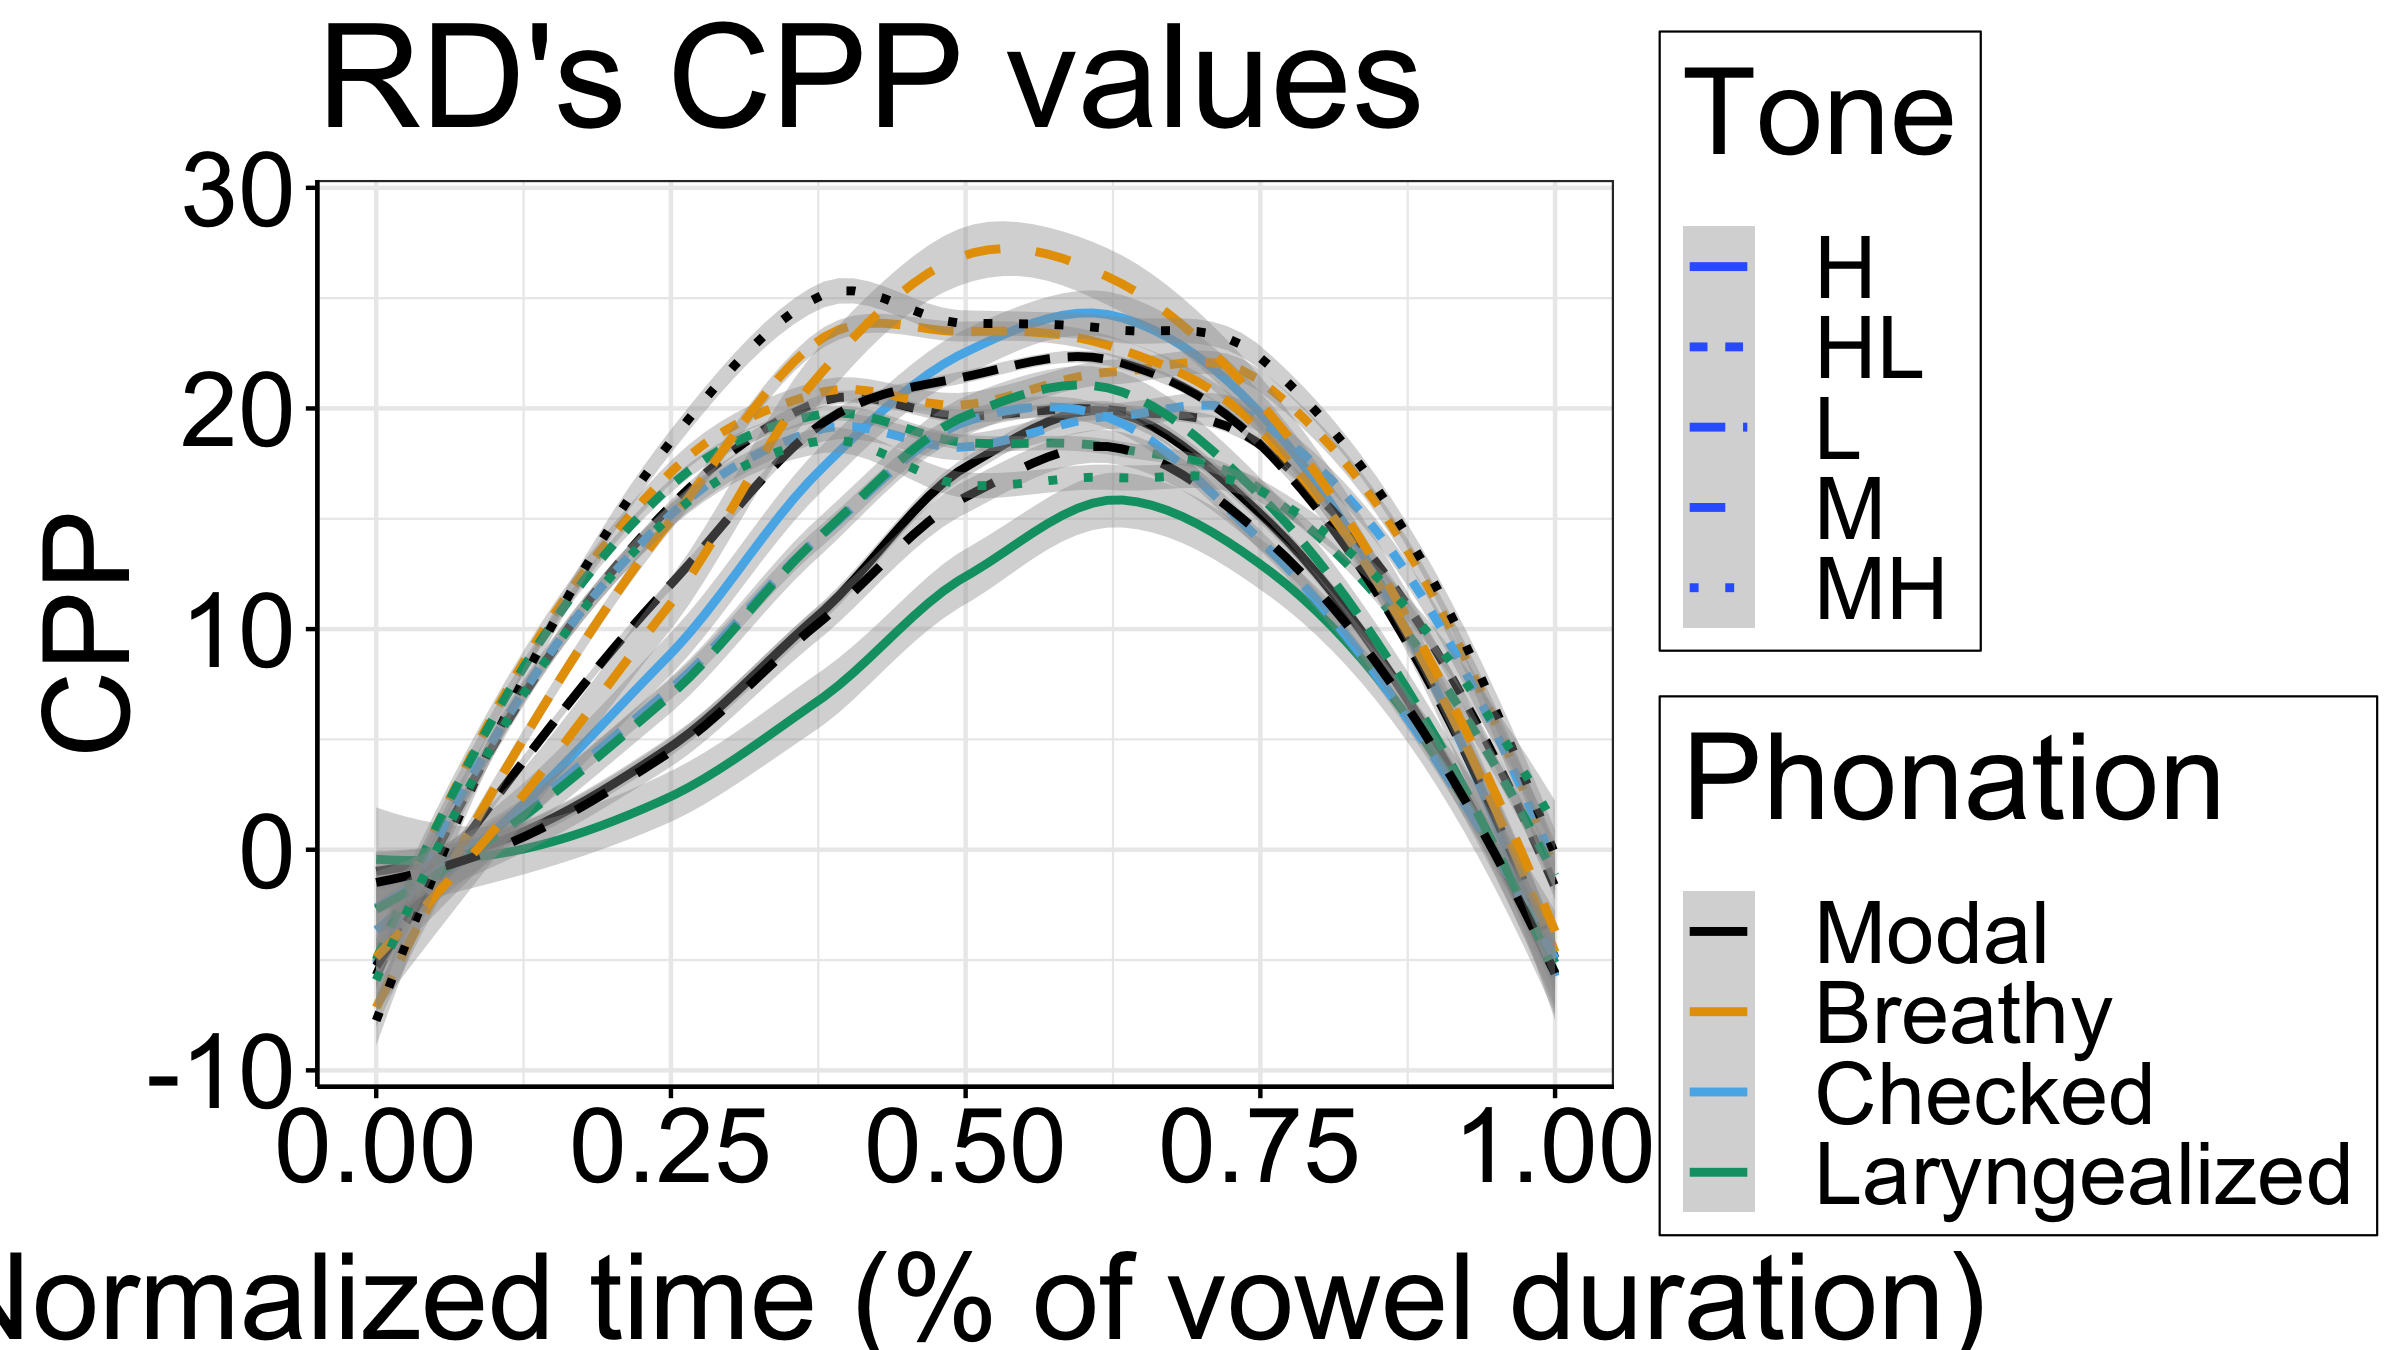
\includegraphics[width=0.9\textwidth]{../RDCPP_line.png}
	\caption{Breathy vowel in the word \textit{ya'} `pound'}
	\label{fig:CheckedVowel}
\end{figure}

Laryngealized vowels are quite common in Zapotecan languages and have received a wide number of different names. Previous descriptions have used terms such as broken, rearticulated, interrupted, and creaky \citep{longDiccionarioZapotecoSan2005,avelinobecerraTopicsYalalagZapotec2004,avelinoAcousticElectroglottographicAnalyses2010,sonnenscheinDescriptiveGrammarSan2005,adlerAcousticsPhonationTypes2016}. In order to avoid confusion, I will use the term laryngealized following \citet{avelinoAcousticElectroglottographicAnalyses2010}. In addition to a wide number of different names these vowels also exhibit a wide range of allophones. 

\citet{avelinoAcousticElectroglottographicAnalyses2010} found in the closely realted Yalálag Zapotec that among his consultants there were at least four different pronunciations as seen in Table~\ref{tab:laryngeal}
\begin{table}[!h]
	\centering
	\caption{Layngealized Vowels in Yalálag Zapotec}
	\label{tab:laryngeal}
	 \begin{tabular}{ll}
	\lsptoprule
	/VˀV/	&  [VʔV]  \\
			&  [VV̰V]   \\
			&  [VV̰ːV̆]  \\
			&  [VV̰V̰]	\\
	\lspbottomrule
	\end{tabular}
\end{table}
In SLZ, each of the consulted language experts would produce this vowel differently. One consultant would do rearticulation, where there is a full glottal stop in the middle of the vowel, or creaky voice. This alternation seemed to be in free variation but there was a greater tendency to creak in low toned words, such as \textit{xa'ag} [ʂa̰ːg] `topil'\footnote{A topil is a type of government office in traditional Oaxacan communities somewhat akin to a sherif. }, see Figure~\ref{fig:FSRLaryngeal} for a comparison between this consultant's pronunciation of the laryngealized vowels.

\begin{figure}[!h]
	\centering
	[INSERT SIDE BY SIDE SPECTROGRAMS]
	\caption{Comparison of FSR's laryngealized vowels in \textit{ya'a} `mountain' and \textit{xa'ag} `topil'}
	\label{fig:FSRLaryngeal}
\end{figure}

The other consultant only ever produces creaky voice for these vowels regardless of the tone with the word. During one of the elicitation sessions, we conducted a sanity check that these were in fact the same vowels and both consultants reliably identified the words and would produce the laryngealized vowel according to their own idiosyncrasies. However, a more detailed perception study is beyond the scope of this paper. 
\begin{figure}[!h]
	\centering
	[INSERT SIDE BY SIDE SPECTROGRAMS]
	\caption{Comparison of RD's laryngealized vowels in \textit{ya'a} `mountain' and \textit{xa'ag} `topil'}
	\label{fig:RDLaryngeal}
\end{figure}

%------------------------------------
\subsection{Tone in SLZ} \label{sec:Tone}
%------------------------------------

As is common among Oto-Manguean languages, SLZ is a tonal languages \citep{suarezMesoamericanIndianLanguages1983,campbellMesoAmericaLinguisticArea1986,silvermanLaryngealComplexityOtomanguean1997,campbellOtomangueanHistoricalLinguistics2017a,campbellOtomangueanHistoricalLinguistics2017}. In SLZ there are five surface tones which appear on a syllable. 


\begin{table}[!h]
	\centering
	\caption{SLZ tones}
	\label{tab:tones}
	 \begin{tabular}{lllll}
	  \lsptoprule
					  % &	 Diacritic  & Example & Transcription \\
	  High   	&  a\supr{H}  &  \textit{xha}   &  [ ʐa\supr{H} ] & `clothing.\textsc{poss}'\\
		Mid    	&  a\supr{M}  &  \textit{lhill} 	& [ ɾiʒ\supr{M} ] & `house.\textsc{poss}' \\
		Low   	&  a\supr{L}  &  \textit{yu'} 	&	 [ juˀ\supr{L} ] & `earth'\\
		Rising	&  a\supr{MH}  &  \textit{yu'u} 	&	[ juˀu\supr{MH} ] & `quicklime (Sp. cal)' \\
		Falling &  a\supr{HL}  &  \textit{yu'u}  &	[juˀu\supr{HL}] &	`house' \\
	  \lspbottomrule
	 \end{tabular}
\end{table}

\begin{figure}[!ht]
	\centering
	\includegraphics[width=0.9\textwidth]{../FSRTonePlot.png}
	\label{fig:FSRTonePlot}
	\caption{Tonal contrasts for FSR averaged and time normalized.}
\end{figure}

\begin{figure}[!ht]
	\centering
	\includegraphics[width=0.9\textwidth]{../RDTonePlot.png}
	\label{fig:RDTonePlot}
	\caption{Tonal contrasts for RD averaged and time normalized.}
\end{figure}

Following discussion from \citet{brinkerhoffTonalPatternsTheir2022} these tones appear to be limited in their distribution. It is true that all five patterns can surface on a syllable but there is a restriction in what tonal patterns are allowed to surface on words that are larger than bimoraic. The patterns that we observe on bimoraic nominals are: HL, MH, and LL. This has the appearance of being a prototypical ``word tone" language following \posscitet{pikeToneLanguagesTechnique1948} categorization. However, recent work from \citet{shihAutosegmentalAimsSurfaceOptimizing2019,mcphersonWordToneEpiphenomenalInpress} has argued that the ``word tone" description is epiphenomenal and can be derived via surface constraints on tone. Which is what \citet{brinkerhoffTonalPatternsTheir2022} argues. 
% \begin{figure}[!ht]
% 	\centering
% 	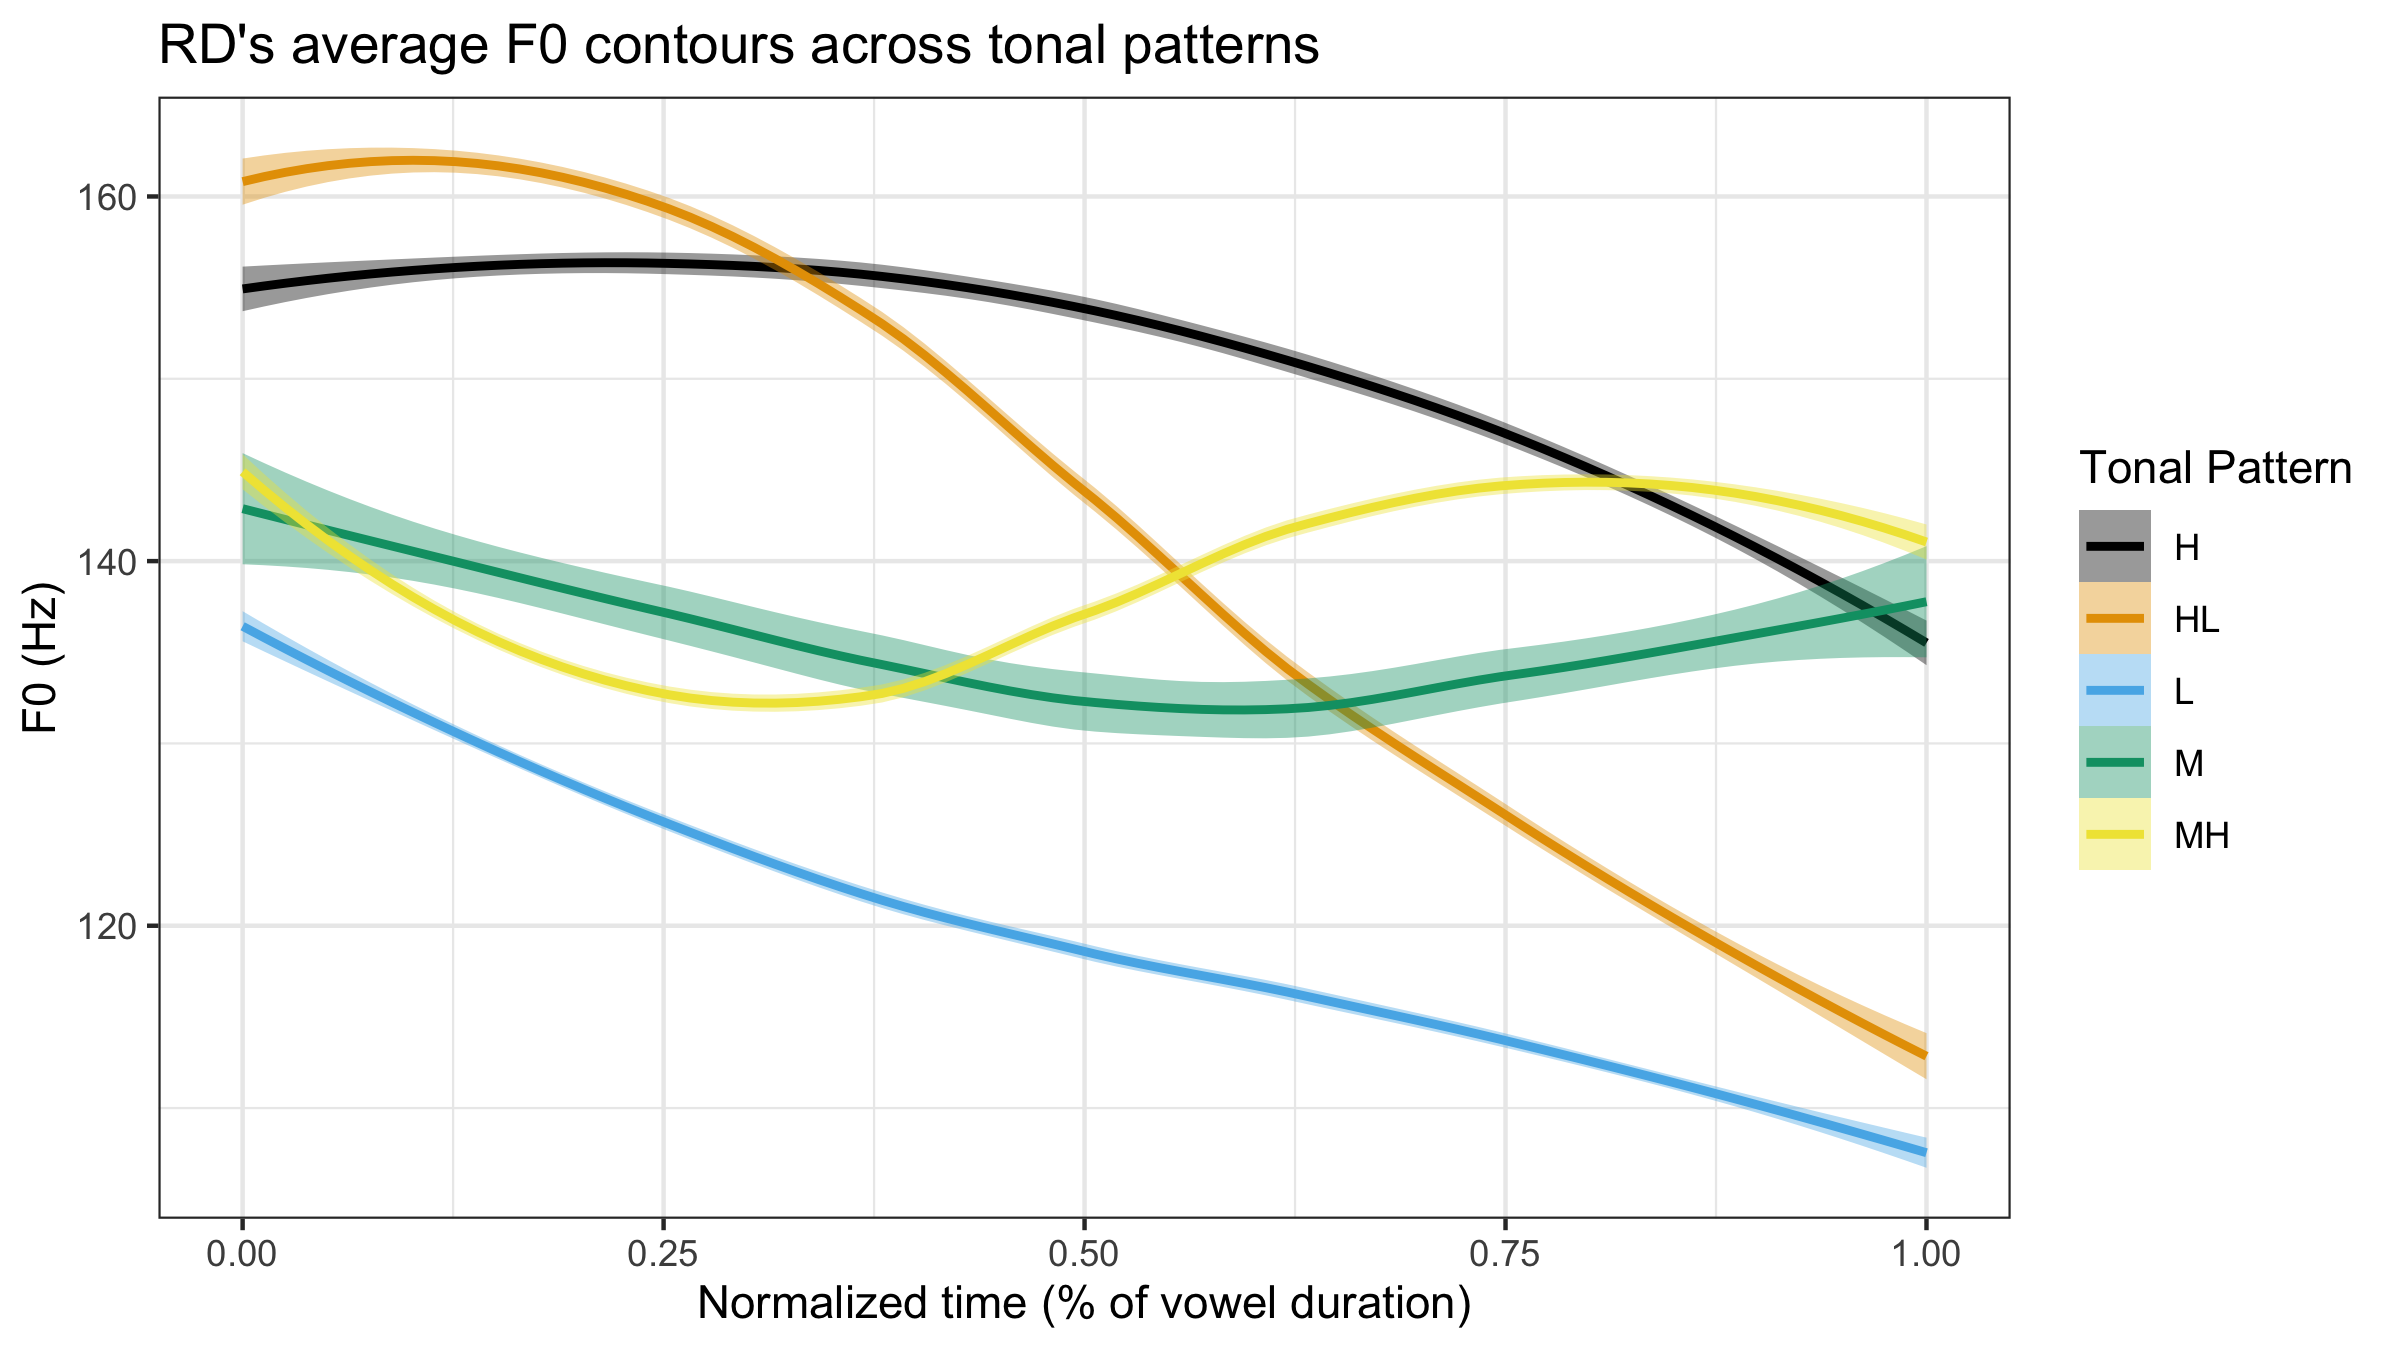
\includegraphics[width=0.9\textwidth]{../JoinTonePlot.png}
% 	\label{fig:LAMNetwork}
% 	\caption{Tonal contrasts for FSR and RD normalized for f0 and time.}
% \end{figure}

%------------------------------------
\section{Interaction of Tone and Phonation} \label{sec:Interaction}
%------------------------------------

Most previous work on the interaction of tone has been focused on the languages of East and Southeast Asia 
\citep[e.g.,][]{masicaDefiningLinguisticArea1976,thurgoodVietnameseTonogenesisRevising2002,yipTone2002,enfieldArealLinguisticsMainland2005,michaudComplexTonesEast2012,brunelleTonePhonationSoutheast2016}. 
What has been found in these descriptions is that certain tones and phonations are codependent (i.e., only occur with each other). For example \citet{smalleyProblemsConsonantsTone1976} and \citet{ratliffMeaningfulToneStudy1992} both describe White Hmong's \textit{-g} tone as being a mid-low tone with breathy phonation and Mandarin's tone 3 is often associated with creaky phonation \citep{hockettPeipingPhonology1947}. \citet{brunelleTonePerceptionNorthern2009} found that creaky phonaiton plays an important role in the production of certain tones. Additionally, work on S'gaw Karen has found that two tones are only differentiated by the presence of some form of amodal phonation (Boehm p.c.). 

However, there has been some observations–especially in Mesoamerican–that tone and phonation can co-vary \citep[e.g,][]{silvermanLaryngealComplexityOtomanguean1997,garellekAcousticConsequencesPhonation2011}. This means that tone can independently occur with any phonation type. This has also been extensively described in multiple Zapotecan languages \citep[e.g.,][]{,avelinobecerraTopicsYalalagZapotec2004,avelinoAcousticElectroglottographicAnalyses2010, chavez-peonInteractionMetricalStructure2010, campbellZenzontepecChatinoAspect2011,villardPhonologyMorphologyZacatepec2015, lopeznicolasEstudiosFonologiaGramatica2016}

\citet{chavez-peonInteractionMetricalStructure2010} has a detailed description of the tone and phonation interactions in San Lucas Quiaviní Zapotec (SLQZ), a central valley variety of Zapotec. The distribution of tone and phonation is found in Table~\ref{tab:SLQZ}. We see that in SLQZ, that both low and falling tone have the full range of possible combinations. However, we see gaps in the high tone for breathy and rising tone can only occur with modal phonation. 

\begin{table}[!ht]
	\centering
	\caption{SLQZ tone and phonation interactions \citep{chavez-peonInteractionMetricalStructure2010}.}
	\label{tab:SLQZ}
	 \begin{tabular}{lcccc}
	  \lsptoprule
					  &	 \textbf{Modal}  & \textbf{Breathy} & \textbf{Creaky} & \textbf{Interrupted} \\
		  High	& ✔︎ & -- & ✔︎ & ✔︎ \\
		  Low & ✔︎ & ✔︎ & ✔︎ & ✔︎ \\
		  Falling & ✔︎ & ✔︎ & ✔︎ & ✔︎ \\
		  Rising & ✔︎ & -- & -- & -- \\
	  \lspbottomrule
	 \end{tabular}
\end{table}

Based on elicitation data collected from 2020-2022, SLZ has a more expansive distribution of tone and phonation when compared to SLQZ but seems to be very similar to other Northern Zapotec varities \citep[e.g.,][]{avelinobecerraTopicsYalalagZapotec2004}. The distribution of SLZ tonal and phonation interactions are given in Table~\ref{tab:ToneVoiceQuality}. 
\begin{table}[!h]
	\caption{Distribution of tone and phonation in SLZ}
	\label{tab:ToneVoiceQuality}
	\centering

	\begin{tabular}{lcccc}
	\lsptoprule
		& \textbf{Modal} & \textbf{Breathy} & \textbf{Checked} & \textbf{Laryngealized} \\
	\hline
	High	& ✔ & -- & ✔ & ✔ \\
	Mid	& ✔ & ✔ & ✔ & ✔\\
	Low	& ✔	& ✔ & ✔ & ✔\\
	High-Low	& ✔	& ✔ & ✔ & ✔\\
	Mid-High	& ✔	& ✔ & -- & ✔ \\
	\lspbottomrule
	\end{tabular}
\end{table}

One of the striking things in this is the lack of high tone with breathy phonation. This gap is interesting because of the long time association of high pitch with breathiness \citep[a good overview–of this association and other phoantion types–is found in][]{eslingVoiceQualityLaryngeal2019}. This gap of breathy phonation and high tone is quite common across the Zapotecan languages (Campbell p.c.). In the case of breathy phonation in SLQZ, \citet{uchiharaToneRegistrogenesisQuiavini2016} offers some convincing evidence that the phonation originated in syllables with low tone and then spread to other tones via analogy. 

%------------------------------------
\section{Acoustic investigation into the phonation} \label{sec:Acoustics}
%------------------------------------

One of the primary ways to measure and investigate phonation is using spectral measures. This has been found to be particularly useful in languages such as Green Hmong \citep{huffmanMeasuresPhonationType1987,andruskiPhonationTypesProduction2000} and Jalapa Mazatec \citep{silvermanPhoneticStructuresJalapa1995,blankenshipTimeCourseBreathiness1997}. Most studies that are using spectral measures are comparing the relative amplitude of different harmonics in the acoustic signals, which has primarily been the difference in the relative amplitude of the first and second harmonics. Other measurements make use of higher harmonics which are closest to the different formants, see Figure~\ref{fig:Harmonics}. 
\begin{figure}[!h]
	\centering
	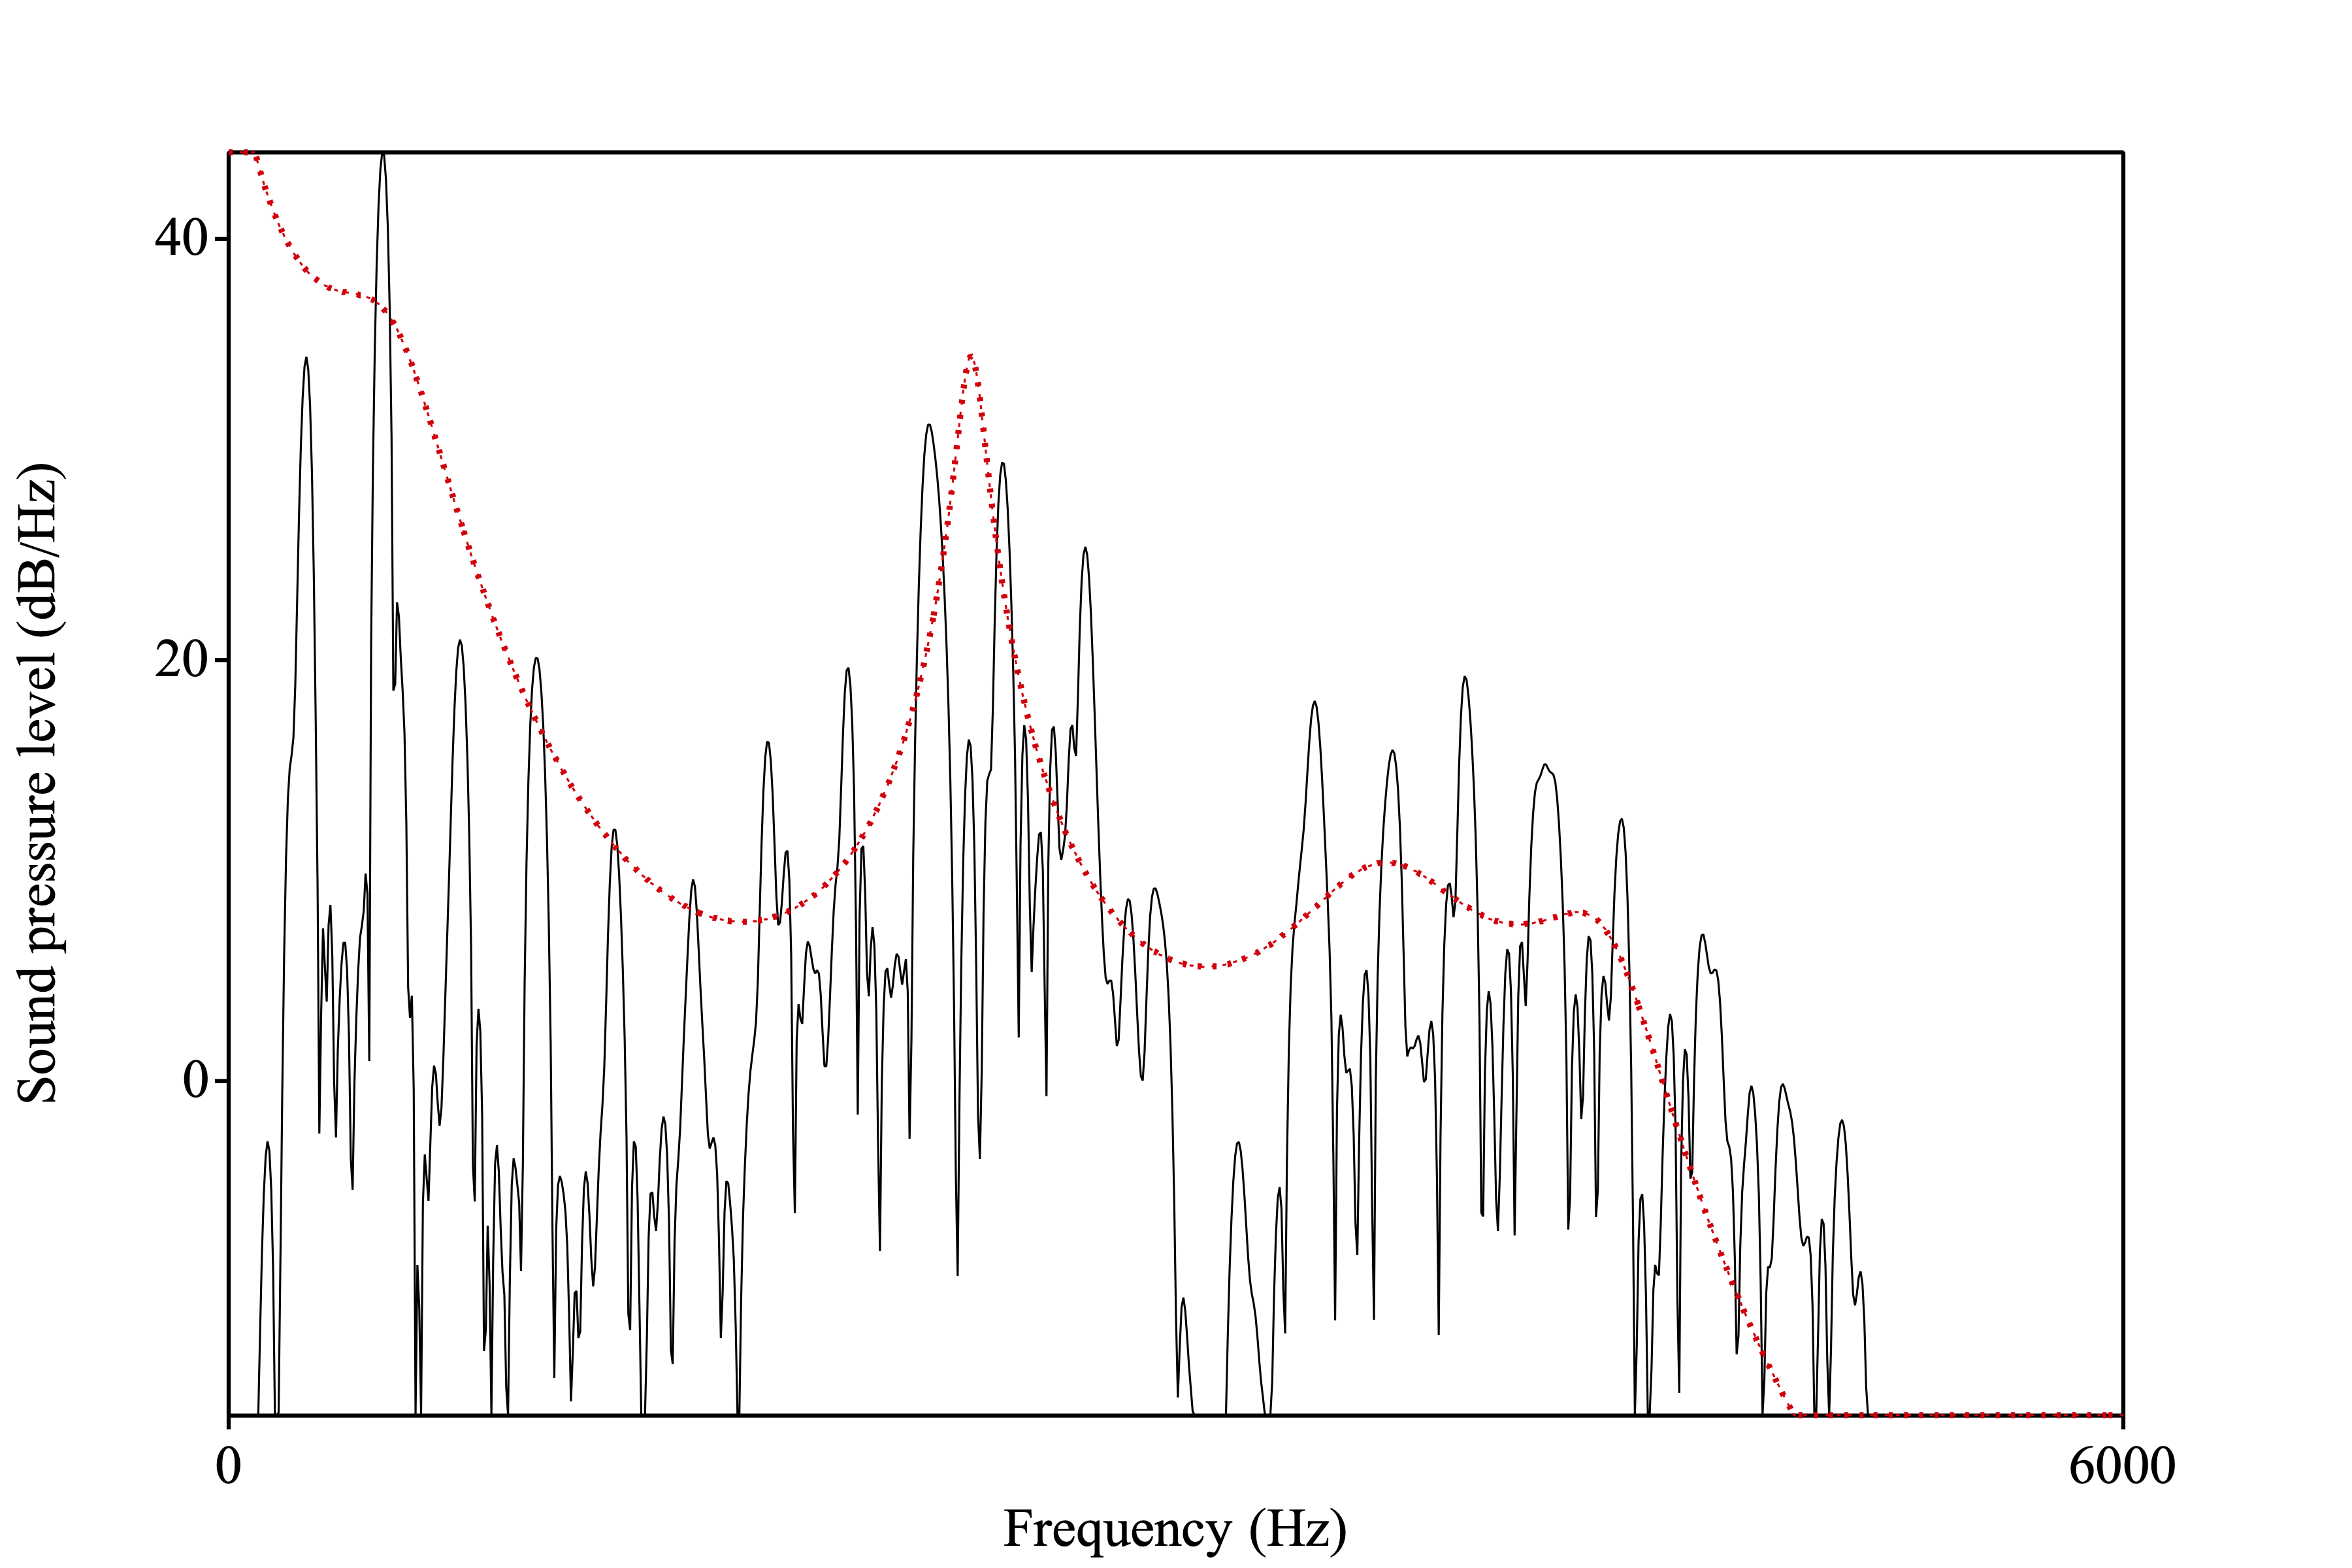
\includegraphics[width=0.9\textwidth]{../Harmonics.png}
	\label{fig:Harmonics}
	\caption{Spectral slice with LPC smoothed line overlaid for the vowel [e]. The harmonics in the spectral slice are represented by each of the dark peaks. The leftmost black solid line peak is the first harmonic (H1) and each subsequent peak represents the next highest harmonic (H2 through H\textit{n}). The red dotted line represents an LPC smoothed line which identifies the formants by the peaks. Each of the harmonics that are closest to the formant peak is identified as A1 through A\textit{n}.}
\end{figure}

When conducting spectral measurements, there are two types of measurements that can be made: corrected and uncorrected. The status of corrected or uncorrected refers to whether or not the influence of formants are taken into account (\cite{garellekPhoneticsVoice2019} provides a good overview of the differences). Most previous studies have not used corrected measure but have been focused on a single vowel /a/ because it minimizes the effects of the first formant \citep{espositoVariationContrastivePhonation2010}. Corrected measures take the formants into account during calculation and minimizes their influences. Fortunately, most software that is used for calculating the acoustic measurements such as VoiceSauce \citep{shueVOICESAUCEProgramVoice2009} and PraatSauce \citep{kirbyPraatSauce2022} produces both corrected and uncorrected values. 

In determining whether or not a given measure corresponds to a given phonation several patterns have been described and validated by many authors. A summary of these findings are given in \citet{garellekPhoneticsVoice2019} where it is noted that when the values of the spectral-tilt measurement are higher than that of the modal's spectral-tilt measurement and the CPP value is lower than the modal's CPP value this more than likely indicates a vowel with breathy phonation. If, however, the spectral-tilt measurements are lower than the modal's spectral-tilt measurements and the CPP value is lower than the modal's CPP value this more than likely indicates a vowel with creaky phonation. This means that if the acoustic measurements for the SLZ phonation types match these findings we can be fairly confident that we are dealing with breathy and creaky phonation. 

The rest of this section will describe the methods, results, and discussion of an acoustic analysis into SLZ's phonation. 

%------------------------------------
\subsection{Methods} \label{sec:Methods}
%------------------------------------

Due to the impact of the COVID-19 pandemic, only two native language speakers of SLZ were able to take part in this study (one male; one female). Both speakers live in Santa Cruz, CA and data collection was done remotely using Zencastr\footnote{\href{https://zencastr.com/}{https://zencastr.com/}}, a professional podcasting website, or in-person outside in a well ventilated location, using a Zoom H4n handheld recorder (44.1kHz, 16-bit). Participates were recorded saying approximately 100 words in the carrier sentence \textit{shnia' X chone las} `I say X three times'. This phrase was repeated three times. 

After the elicitation were completed the audio was uploaded into ELAN \citep{wittenburgELANProfessionalFramework2006} for initial segmentation into sentences. This was then followed by segmenting of the vowel portion in Praat \citep{boersmaPraatDoingPhonetics2021}. These segments were then inputted to VoiceSauce \citep{shueVOICESAUCEProgramVoice2009} were each vowel was resampled at 16kHZ for acoustic measurement. The acoustic measurements of VoiceSauce were then analyzed in R \citep{rcoreteamLanguageEnvironmentStatistical2021}. In order to investigate the differences in timing, each vowel was normalized for time.

%------------------------------------
\subsection{Spectral-tilt results} \label{sec:Results}
%------------------------------------

The results of the spectral-tilt measurements were for the most part accurate. As noted by \citet{espositoVariationContrastivePhonation2010} for a Central Valley Zapotec, there is a difference in which acoustic measurements were most informative for the speakers based on their sex. Similar to \citeauthor{espositoVariationContrastivePhonation2010}, the female speaker was best characterized with the H1-H2 measurements and the male speaker was best characterized with H1-A3. For the female speaker this was true for all phonation types except for breathy voice which measured similarly to the other non-modal vowels. This is not too unsurprising considering the fact that the female speaker would more often produce a full glottal fricative in these environments than a breathy vowel. This can be seen in Figure~\ref{fig:FSRh1h2} where the modal vowel is represented by the solid black line. All other lines which represent breathy, checked, and laryngealized are all lower than that of the modal. 
\begin{figure}[!ht]
	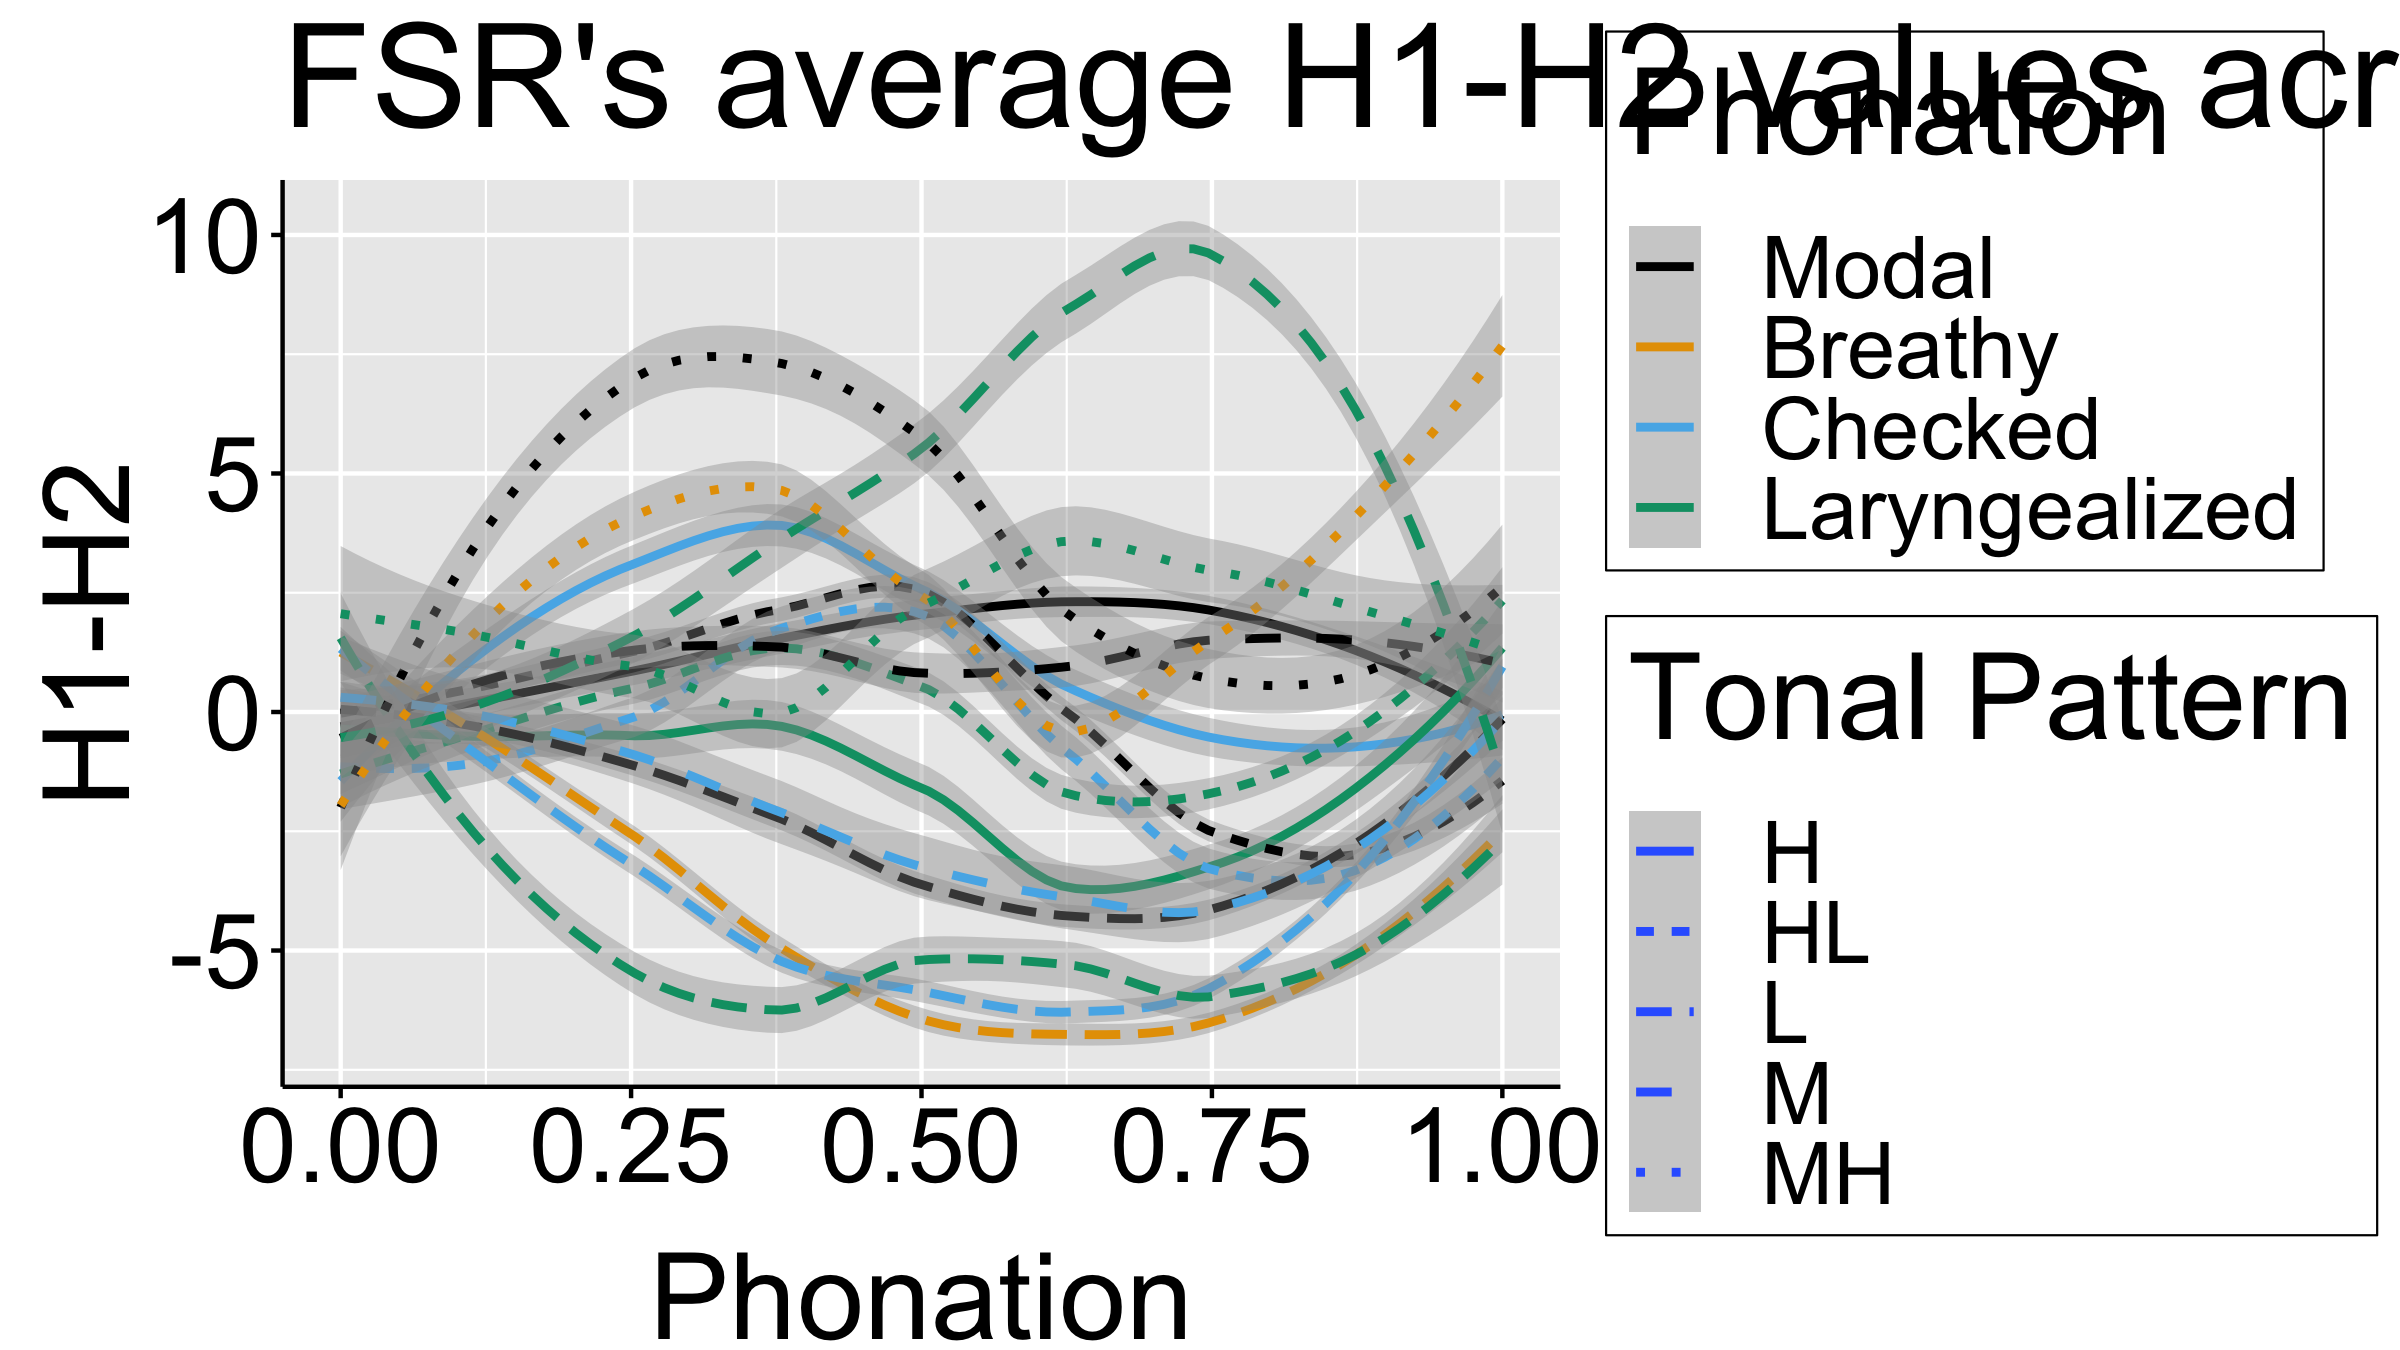
\includegraphics[width=0.9\textwidth]{../h1h2_line_L.png}
	\caption{FSR's H1-h2 values.}
	\label{fig:FSRh1h2} 
\end{figure}

As mentioned previously, one of our speakers would regularly produce the laryngealized vowels with rearticulation, meaning that they produced the vowel with glottalization, with either creakiness or a full glottal closure, in the middle of the vowel. This is in contrast with the checked vowels which have a short period of creakiness or a full glottal closure at the end of the vowel. This means that our spectral-tilt measurements should reflect a difference in time with creaky voice appearing earlier in the laryngealized vowels than checked vowels. In Figure~\ref{fig:FSRh1h2checked}, the spectral-tilt values for laryngealized and checked vowels are plotted along a time normalized scale. The important thing to be aware of is the difference in where the lowest part of the plot is located. For checked vowels, represented by the solid lines, the lowest part of the spectral-tilt measurement is located in the last quarter of the vowel. This dip, however, occurs earlier in the vowel for the laryngealized vowels closer halfway to 75\% of the vowel. 
\begin{figure}[!ht]
	\includegraphics[width=0.9\textwidth]{../h1h2_CheckedLaryngeal.png}
	\caption{FSR's H1-h2 values for checked and laryngealized.}
	\label{fig:FSRh1h2checked} 
\end{figure}

As mentioned mentioned previously, the results of the spectral analysis for the male SLZ speaker were inconclusive in terms of H1-H2. As seen in Figure~\ref{fig:RDh1h2} all of the different phonation types are essentially identical with less than 1 dB difference between the different phonation types. 
\begin{figure}[!ht]
	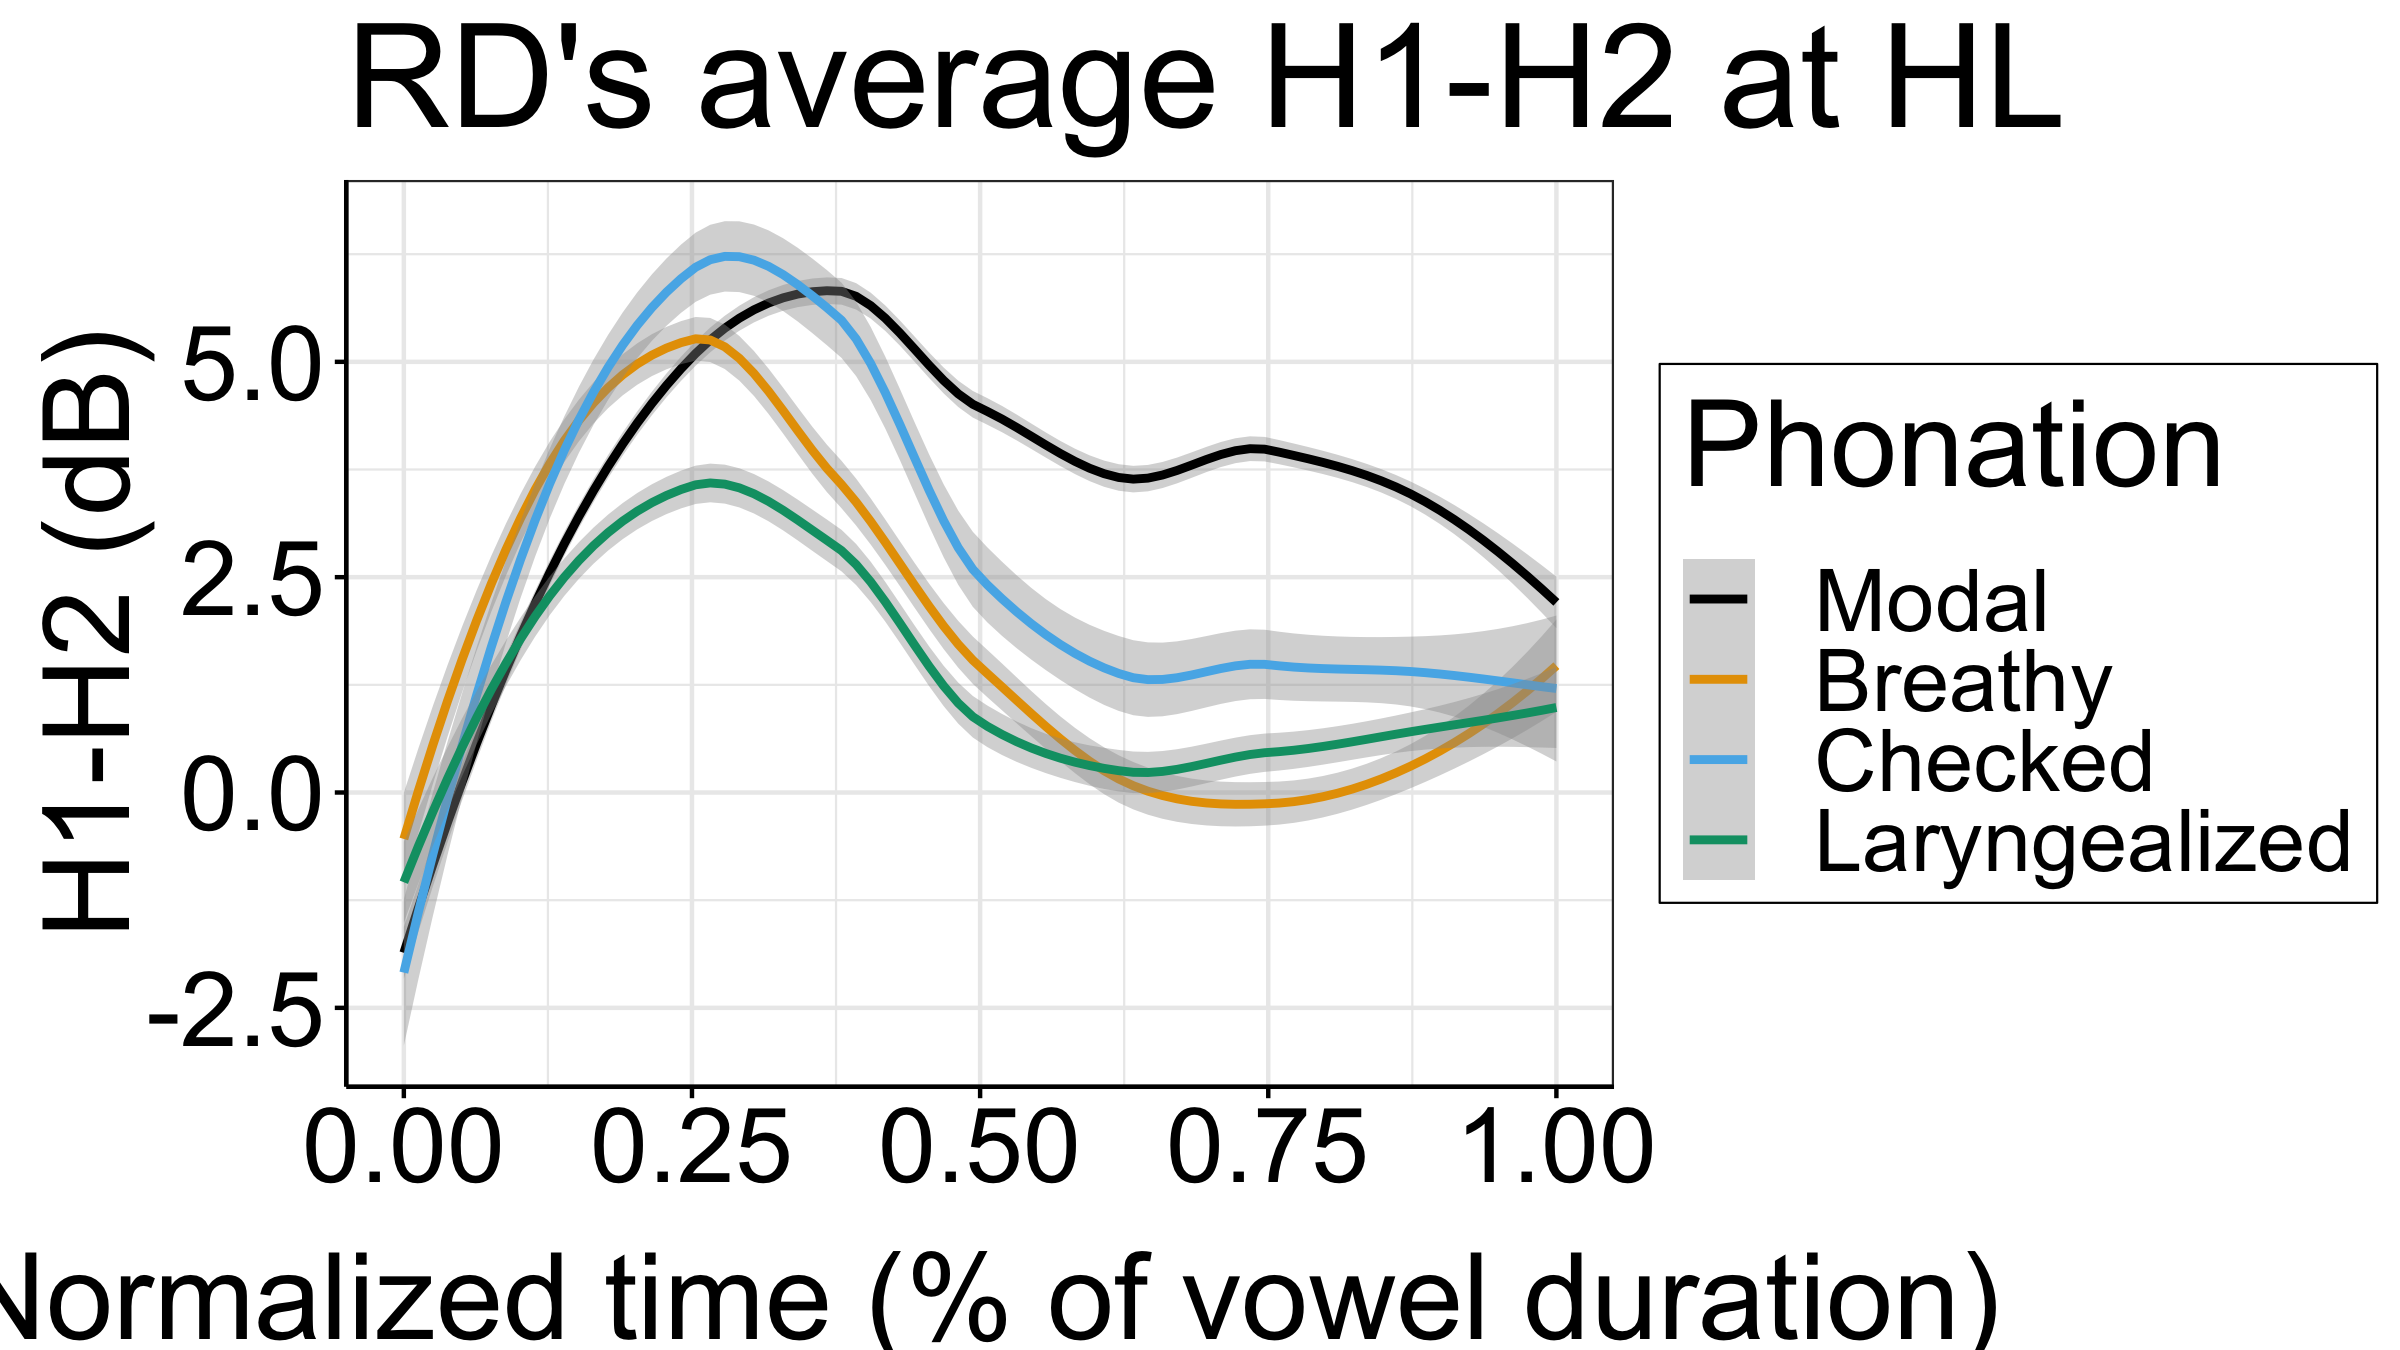
\includegraphics[width=0.9\textwidth]{../RDh1h2_line_HL.png}
	\caption{RD's H1-H2 values in HL toned syllables.}
	\label{fig:RDh1h2} 
\end{figure}
The H1-A3 spectral measures, however, show the expect patterns, as seen in Figure~\ref{fig:RDh1a3}. 
\begin{figure}[!ht]
	\includegraphics[width=0.9\textwidth]{../RDH1A3_HL.png}
	\caption{RD's total H1-A3 values in HL toned syllables. }
	\label{fig:RDh1a3} 
\end{figure}

%------------------------------------
\subsection{Statistical results} \label{sec:Stats}
%------------------------------------
In order to determine whether or not the gestures for pitch and phonation are overlapping a mixed-effects linear regression analysis was performed. Following \citet{garellekAcousticConsequencesPhonation2011}, the results for both speaker were combined together and then divided into thirds based on the normalized times. This allows for analysis of each third of the vowel to determine if the phonation and pitch gestures are overlapping. To this effect, the F0 measurements where treated as the dependent variable with speaker treated as random. The results of the analysis showed that the phonation categories, spectral-tilt measurements, and CPP all had an effect in different portions of the vowel. Specifically the portions of the analysis showed that did not show any effects where the first-third of the vowel for CPP and the last third for the laryngealized category.


%------------------------------------
\subsection{Discussion of the results} \label{sec:Discussion}
%------------------------------------

%------------------------------------
\section{Challenges to theories} \label{sec:Challenges}
%------------------------------------

\begin{itemize}
	\item How does this support or detract from \posscitet{silvermanLaryngealComplexityOtomanguean1997} claims?
	\begin{itemize}
		\item Do we see the gestural timing that \citet{silvermanLaryngealComplexityOtomanguean1997} claims to exist?
	\end{itemize}
	\item Issues with breathy not present with H. 
	\item Additionally there is this question about why we are seeing laryngealized vowels in H tone
	\begin{itemize}
		\item Could \posscitet{eslingVoiceQualityLaryngeal2019} model of interactions be used to explain what we are seeing?
	\end{itemize}
\end{itemize}

%------------------------------------
\section{Conclusion} \label{sec:Conclusion}
%------------------------------------

%------------------------------------
%BIBLIOGRAPHY
%------------------------------------

%\singlespacing
% \nocite{*}
\printbibliography[heading=bibintoc]

\end{document} 